\chapter{Physical Design Implementation}
\label{chap:physical_design}

After logic synthesis, the gate-level netlist was imported into the OpenROAD engine through the OpenLane2 flow for physical implementation. This stage transforms the logical design into a manufacturable layout by determining standard cell locations, constructing the clock network, and routing signal interconnections. Using the SkyWater SKY130 PDK, OpenLane2 automatically performed floorplanning, placement, clock tree synthesis (CTS), global routing, and detailed routing.

\begin{figure}[!htbp]
    \centering
    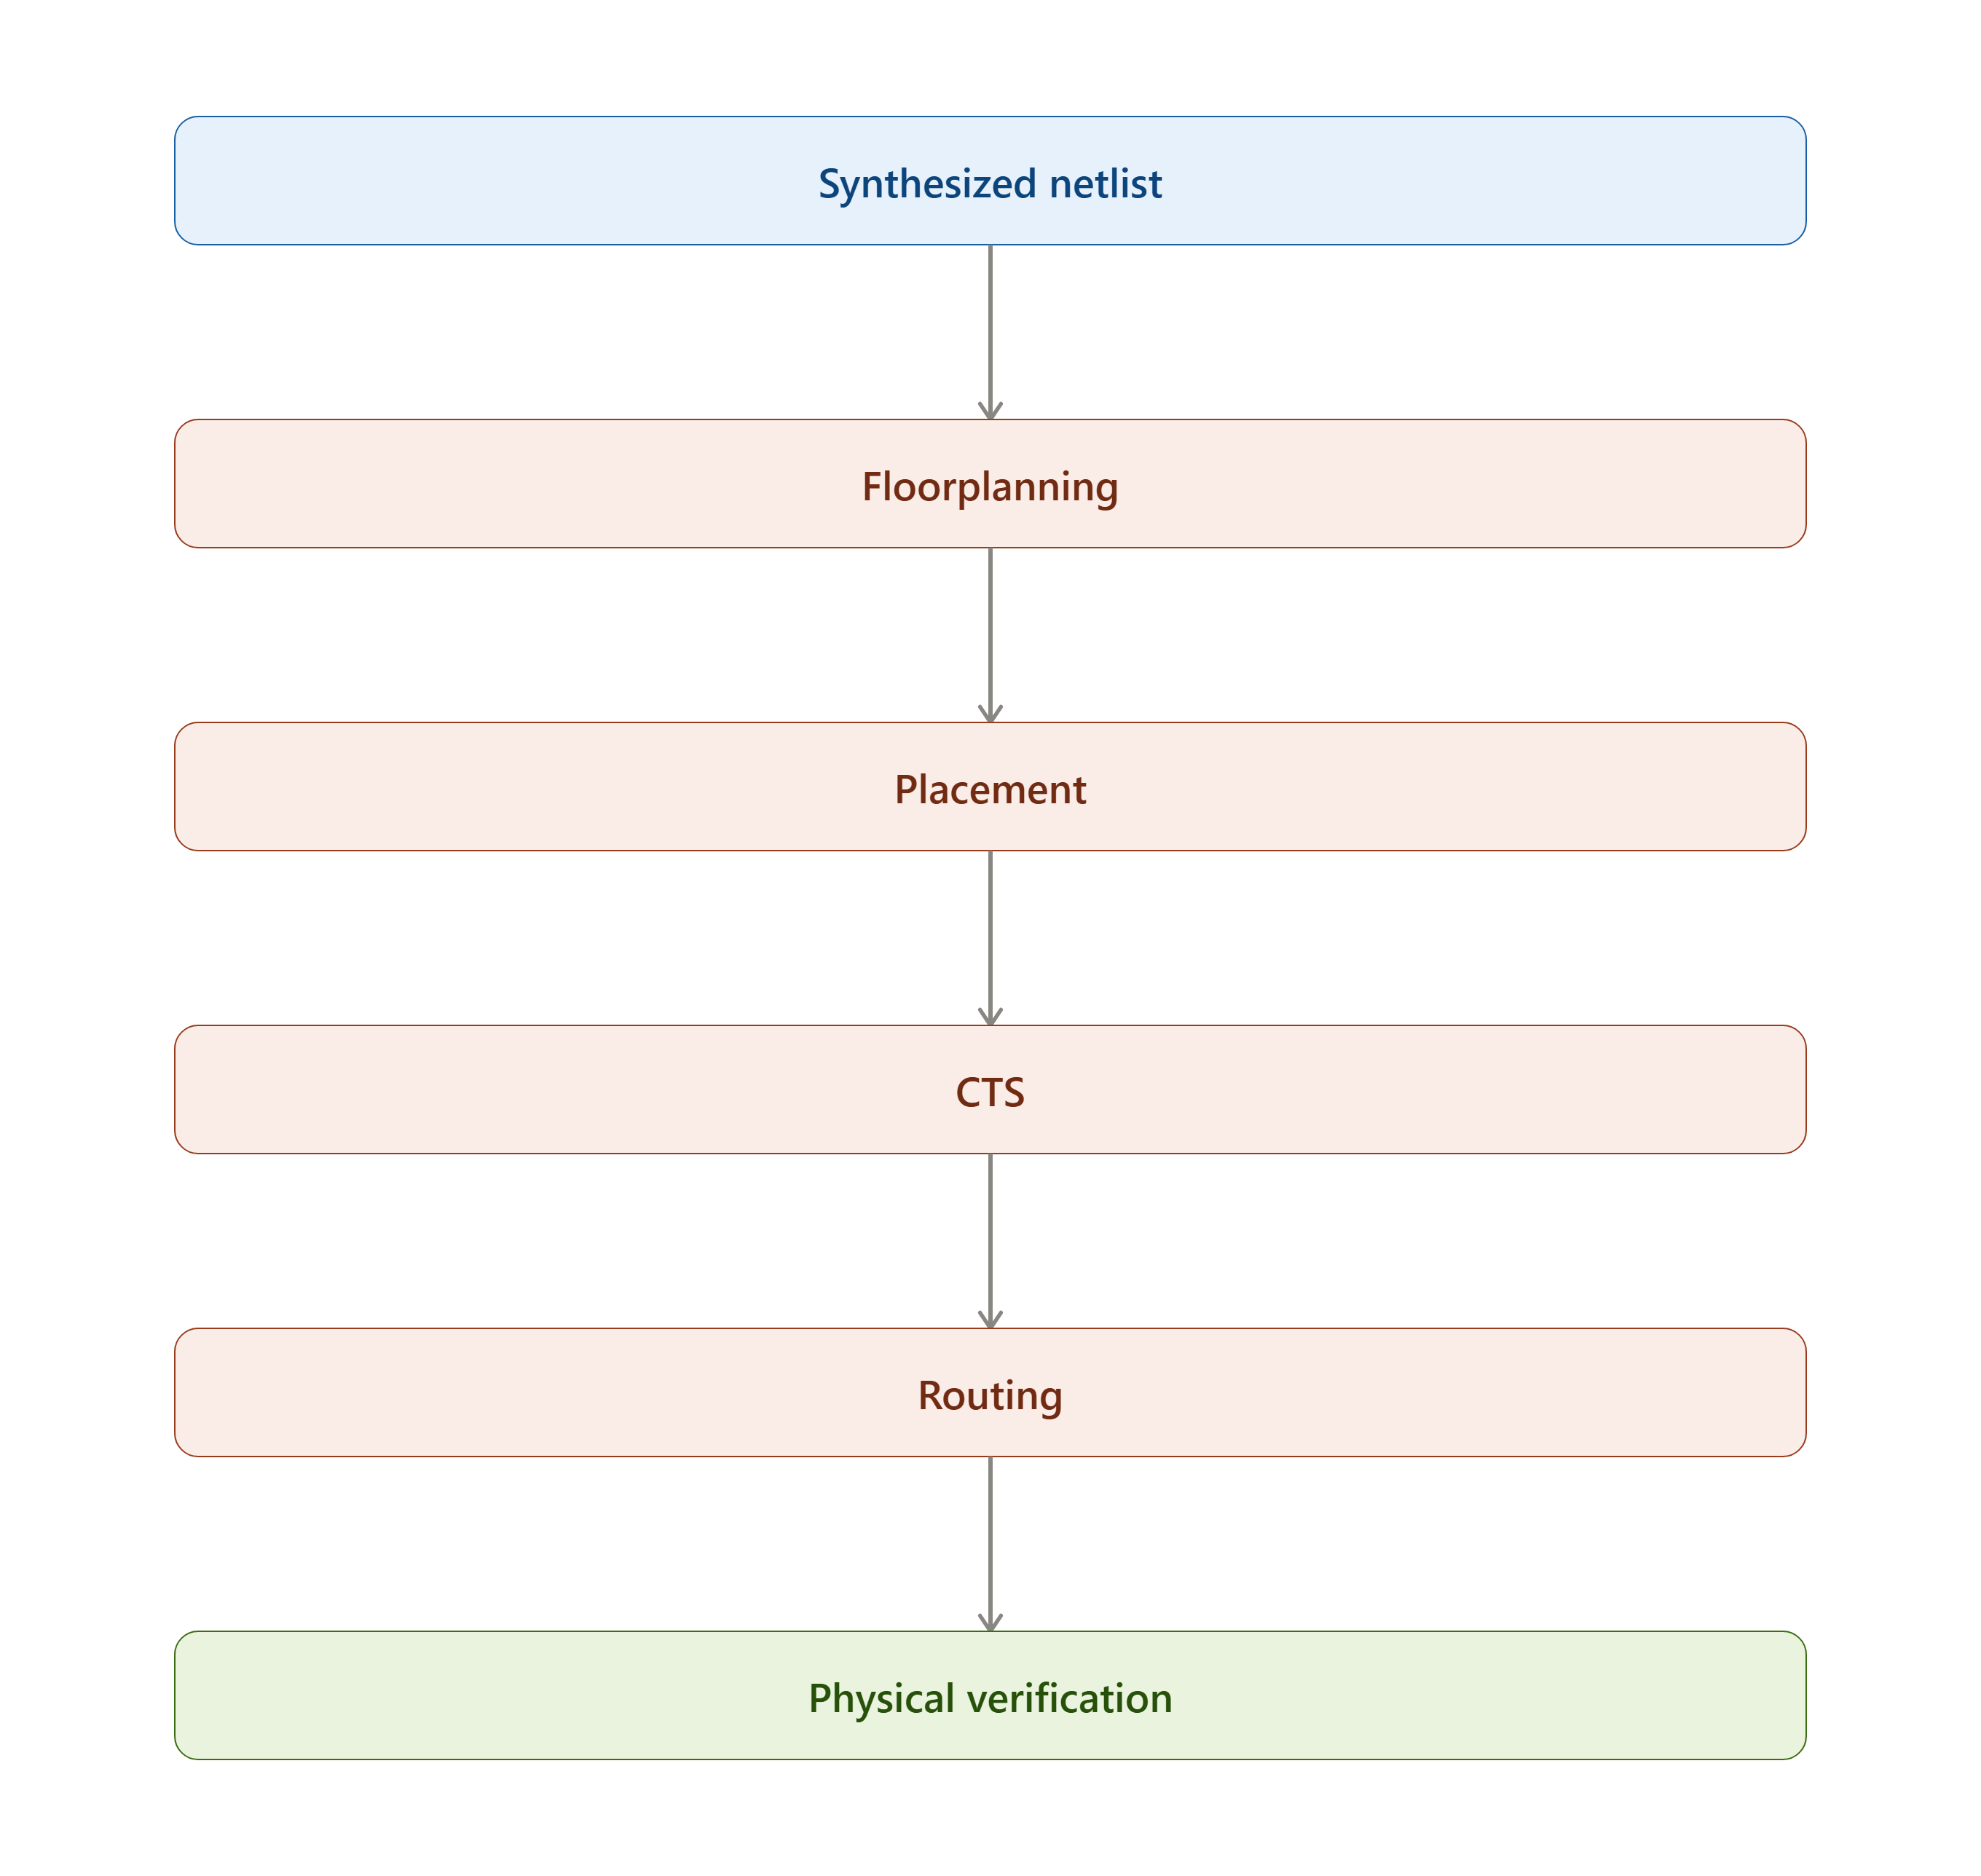
\includegraphics[width=0.88\textwidth]{images/physical_design_flow.png}
    \caption{Physical design implementation flow using OpenROAD.}
    \label{fig:physical_design_flow}
\end{figure}


%%%%%%%%%%%%%%%%%%%%%%%%%%%%%%%%%%%%%%%%%%%%%%%%%%%%%%%%%%%%%%%

\section{Floorplanning}

Floorplanning is the first stage of physical implementation where the die area, core area, placement rows, utilization, and I/O pin locations are established. A well-planned floorplan provides sufficient routing resources and minimizes congestion during later stages of implementation.

Figure~\ref{fig:floorplan} shows the generated floorplan of the UART IP core obtained from OpenROAD.

\begin{figure}[!htbp]
    \centering
    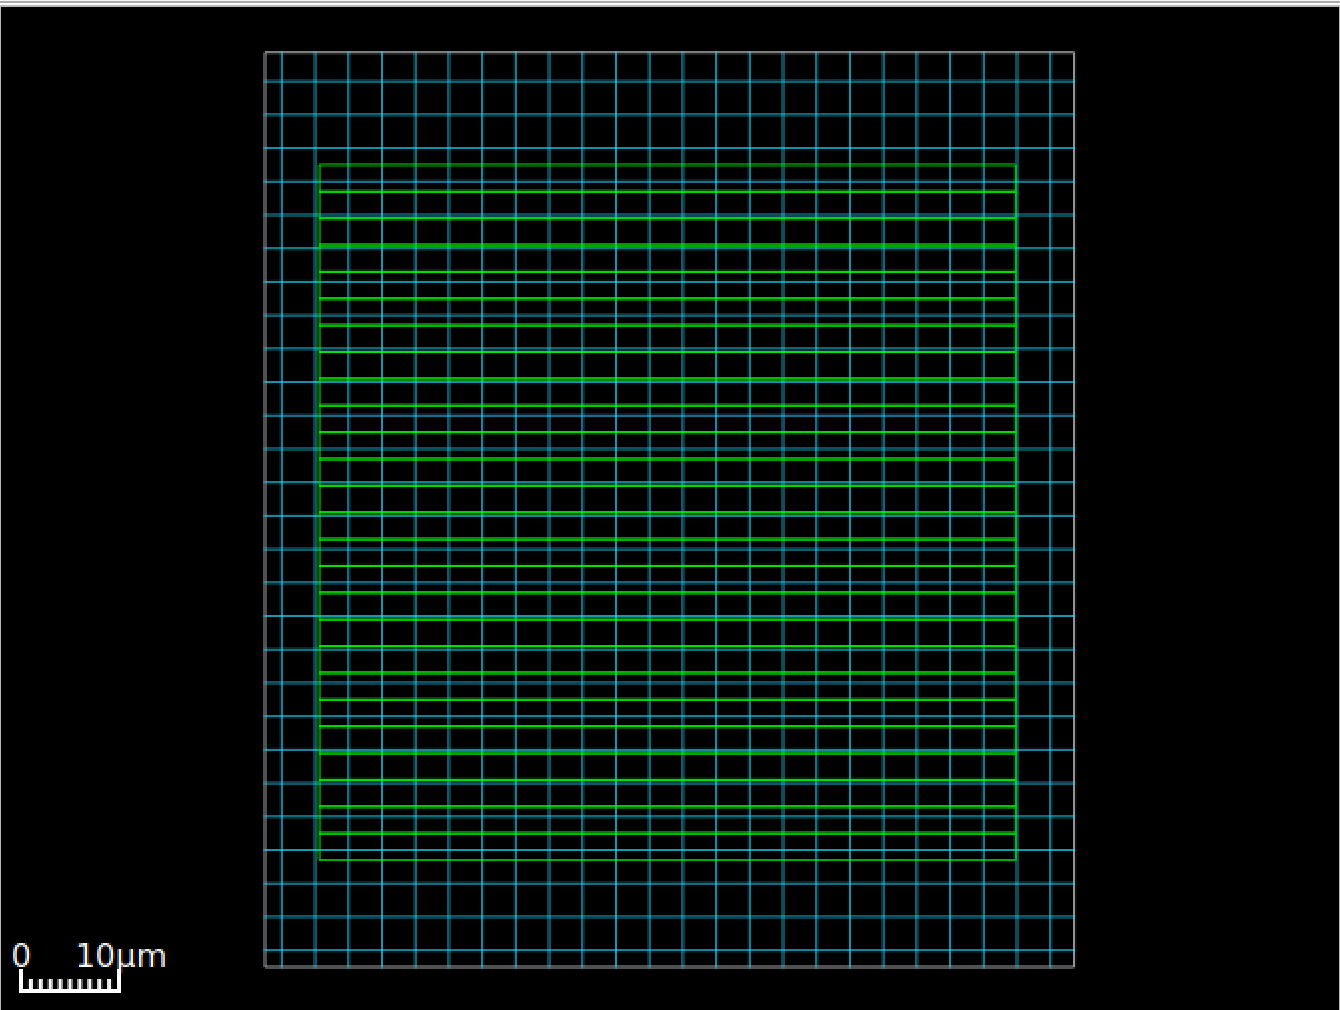
\includegraphics[width=0.93\textwidth]{images/Standard_Cell_Rows_Generated_During_Floorplanning.png}
    \caption{Generated floorplan of the UART ASIC design.}
    \label{fig:floorplan}
\end{figure}

The floorplanning report generated during implementation is summarized in Table~\ref{tab:floorplan_metrics}.

\begin{table}[!htbp]
\centering
\caption{Floorplanning metrics}
\label{tab:floorplan_metrics}
\begin{tabular}{lc}
\toprule
Parameter & Value\\
\midrule
Die Area & 7658.18 $\mu m^2$\\
Core Area & 5009.80 $\mu m^2$\\
Standard Cell Area & 3210.58 $\mu m^2$\\
Instance Count & 375\\
Core Utilization & 64.09\%\\
I/O Pins & 25\\
\bottomrule
\end{tabular}
\end{table}

The generated floorplan achieved a core utilization of approximately 64\%, providing sufficient whitespace for placement optimization and routing while maintaining an efficient silicon area.

%%%%%%%%%%%%%%%%%%%%%%%%%%%%%%%%%%%%%%%%%%%%%%%%%%%%%%%%%%%%%%%

\section{Global and Detailed Placement}

After floorplanning, OpenROAD performs global placement to determine approximate locations of all standard cells while minimizing wirelength and improving timing. This is followed by detailed placement, where every standard cell is aligned to legal placement rows and overlap violations are removed.

Figure~\ref{fig:placement} shows the placed standard-cell layout generated during the placement stage.

\begin{figure}[!htbp]
    \centering
    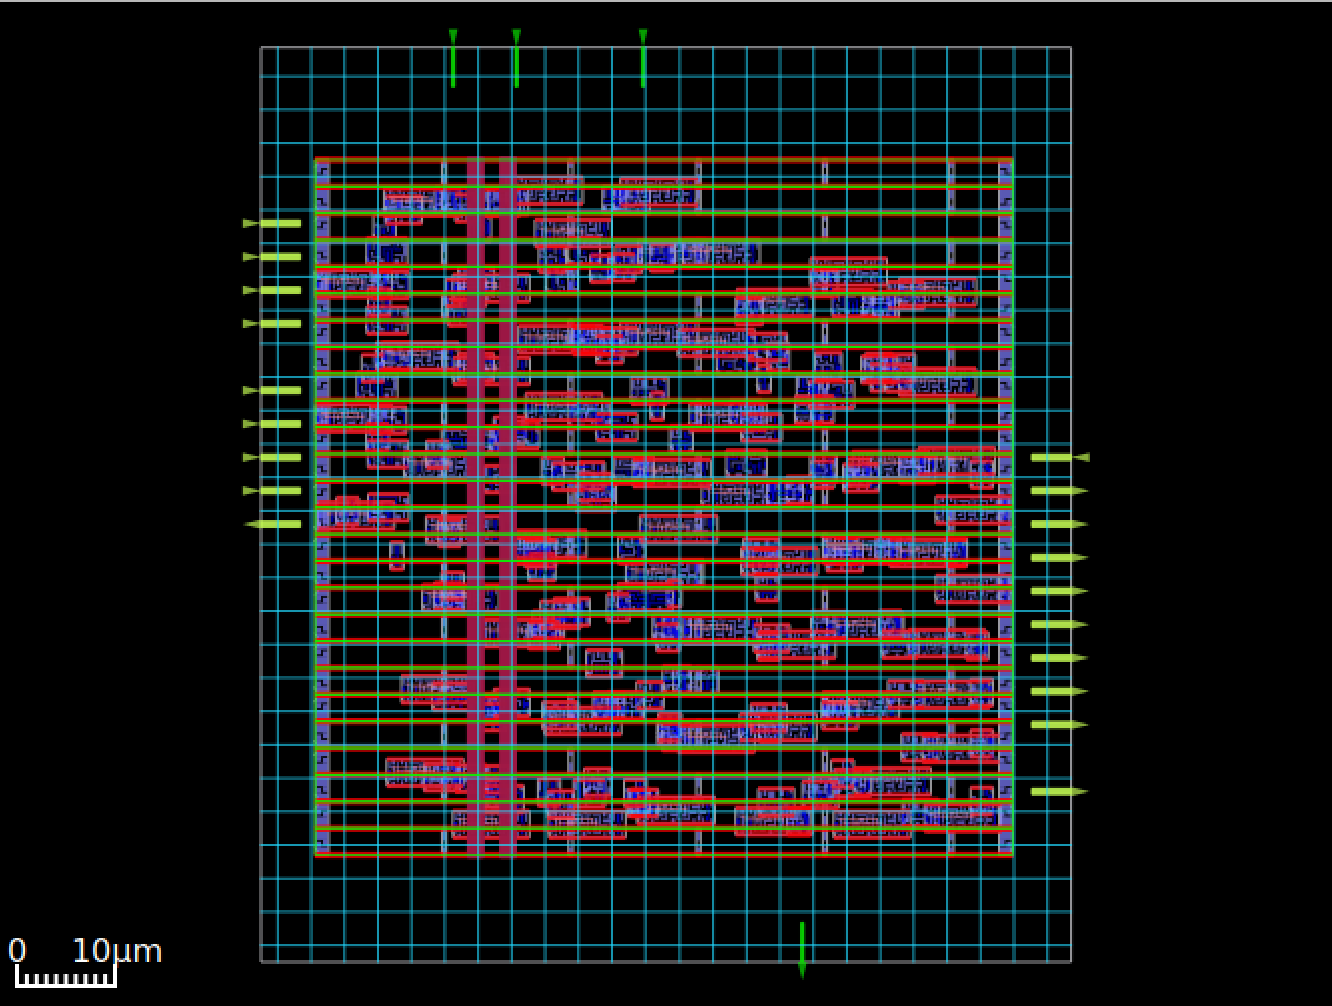
\includegraphics[width=0.93\textwidth]{images/Standard_Cell_Placement.png}
    \caption{Standard-cell placement generated by OpenROAD.}
    \label{fig:placement}
\end{figure}

The placement statistics obtained from the OpenLane2 implementation are summarized in Table~\ref{tab:placement_metrics}.

\begin{table}[H]
\centering
\caption{Placement metrics}
\label{tab:placement_metrics}
\begin{tabular}{lc}
\toprule
Parameter & Value\\
\midrule
Total Displacement & 0.0 $\mu$m\\
Average Displacement & 0.0 $\mu$m\\
Maximum Displacement & 0.0 $\mu$m\\
HPWL Before Optimization & 3351.5 $\mu$m\\
HPWL After Optimization & 3207.2 $\mu$m\\
HPWL Improvement & 4.3\%\\
Standard Cell Utilization & 51.65\%\\
\bottomrule
\end{tabular}
\end{table}

OpenROAD also inserted additional cells required for placement legalization and timing optimization. The resulting cell distribution is shown in Table~\ref{tab:placement_cells}.

\begin{table}[H]
\centering
\caption{Cell distribution after detailed placement}
\label{tab:placement_cells}
\begin{tabular}{lc}
\toprule
Cell Type & Count\\
\midrule
Sequential Cells & 55\\
Combinational Cells & 156\\
Timing Repair Buffers & 31\\
Tap Cells & 70\\
Fill Cells & 52\\
Inverters & 8\\
Total Cells & 372\\
\bottomrule
\end{tabular}
\end{table}

The detailed placement stage completed without overlap violations. The reported zero displacement indicates that all standard cells were successfully legalized while preserving the optimized placement generated during global placement. Furthermore, the reduction in Half-Perimeter Wire Length (HPWL) after optimization demonstrates improved routing efficiency and timing quality.


%%%%%%%%%%%%%%%%%%%%%%%%%%%%%%%%%%%%%%%%%%%%%%%%%%%%%%%%%%%%%%%

\section{Clock Tree Synthesis}

Clock Tree Synthesis (CTS) is performed after placement to distribute the clock signal uniformly to all sequential elements while minimizing clock skew, insertion delay, and timing violations. During this stage, OpenROAD inserts clock buffers and inverters to construct an optimized clock distribution network.

Figure~\ref{fig:cts} shows the CTS stage.

\begin{figure}[!htbp]
    \centering
    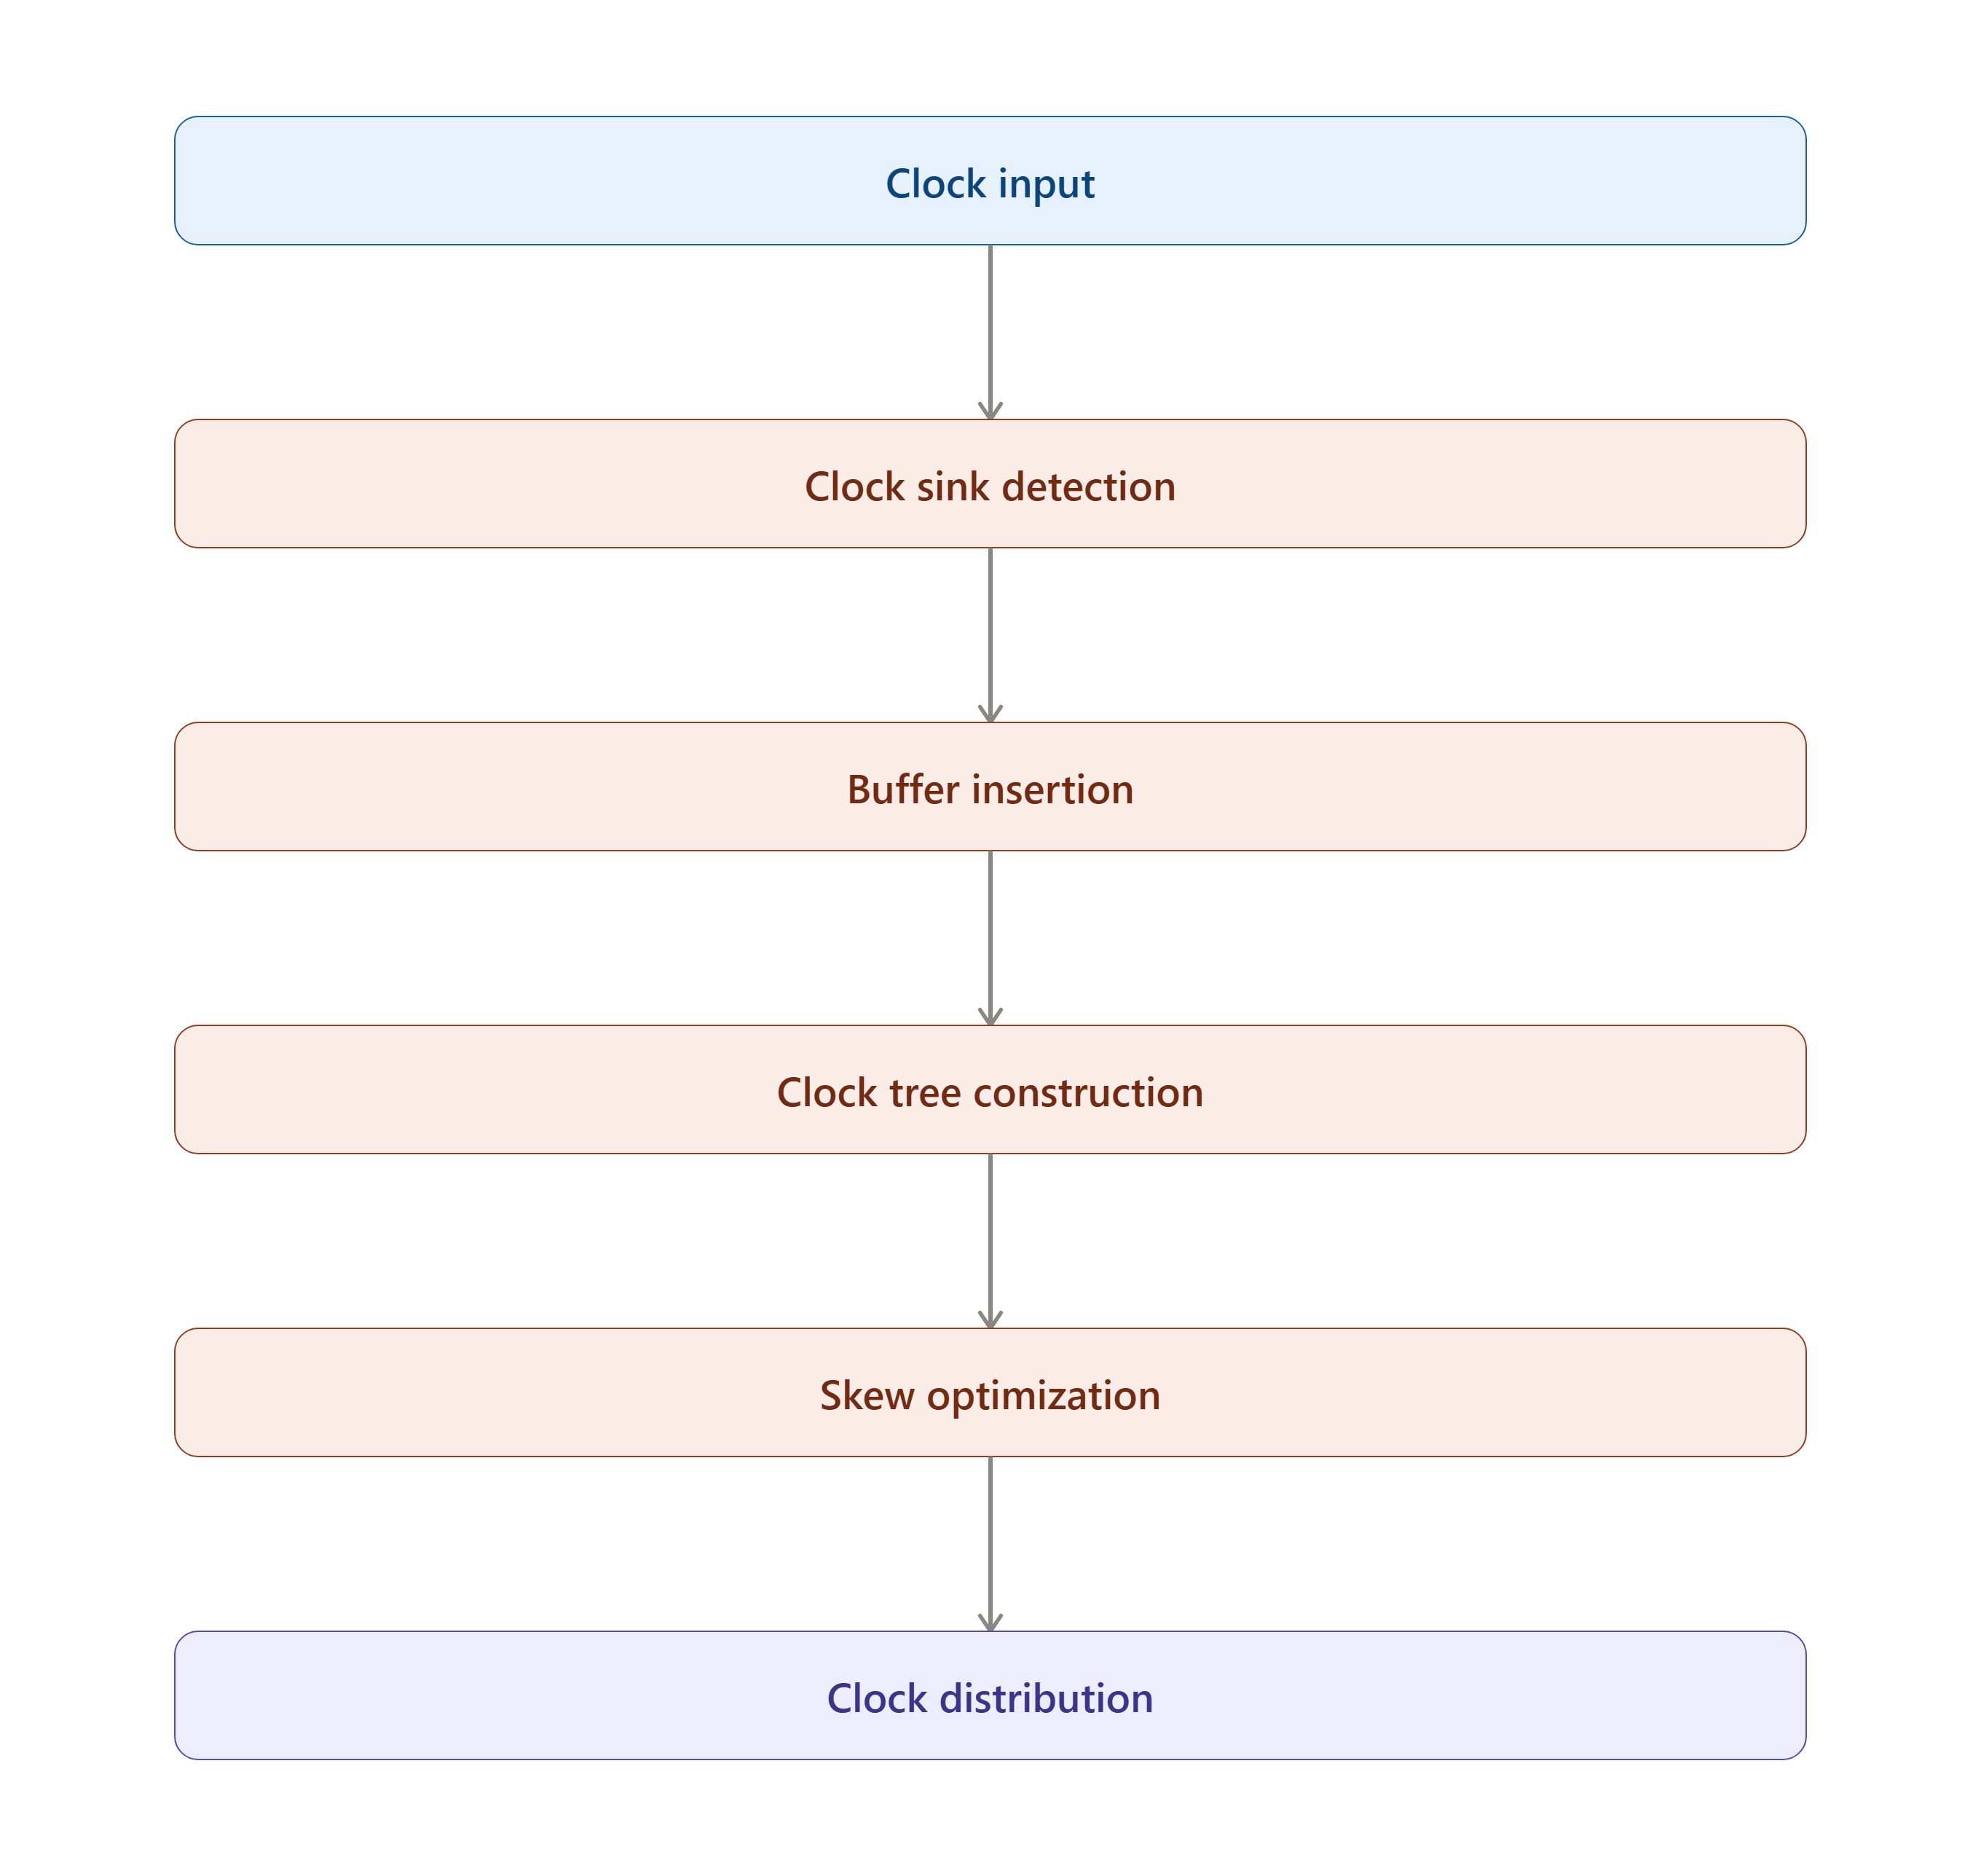
\includegraphics[width=0.93\textwidth]{images/clock_tree_synthesis.png}
    \caption{Clock Tree Synthesis (CTS) stages.}
    \label{fig:cts}
\end{figure}

The CTS report generated during implementation is summarized in Table~\ref{tab:cts_metrics}.

\begin{table}[H]
\centering
\caption{Clock Tree Synthesis statistics}
\label{tab:cts_metrics}
\begin{tabular}{lc}
\toprule
Parameter & Value\\
\midrule
Clock Nets & 6\\
Clock Buffers Inserted & 5\\
Clock Inverters Inserted & 3\\
Timing Repair Buffers & 78\\
Sequential Cells & 55\\
Total Cell Instances & 427\\
Total Cell Area & 3405.77 $\mu m^2$\\
Core Utilization & 64.09\%\\
\bottomrule
\end{tabular}
\end{table}

The CTS stage successfully generated the clock distribution network without introducing clock-related violations. The insertion of dedicated clock buffers and inverters balanced the clock paths while maintaining acceptable utilization. Additional timing repair buffers were inserted automatically by OpenROAD to improve timing performance before routing.


%%%%%%%%%%%%%%%%%%%%%%%%%%%%%%%%%%%%%%%%%%%%%%%%%%%%%%%%%%%%%%%

\section{Global and Detailed Routing}

Following Clock Tree Synthesis (CTS), OpenROAD performs routing to establish all electrical connections between the placed standard cells. The routing process consists of two stages: global routing, which determines approximate routing paths, and detailed routing, which generates the final metal interconnections while satisfying the SKY130 design rules.

Figure~\ref{fig:routing} shows the routed layout generated after the completion of detailed routing.

\begin{figure}[!htbp]
    \centering
    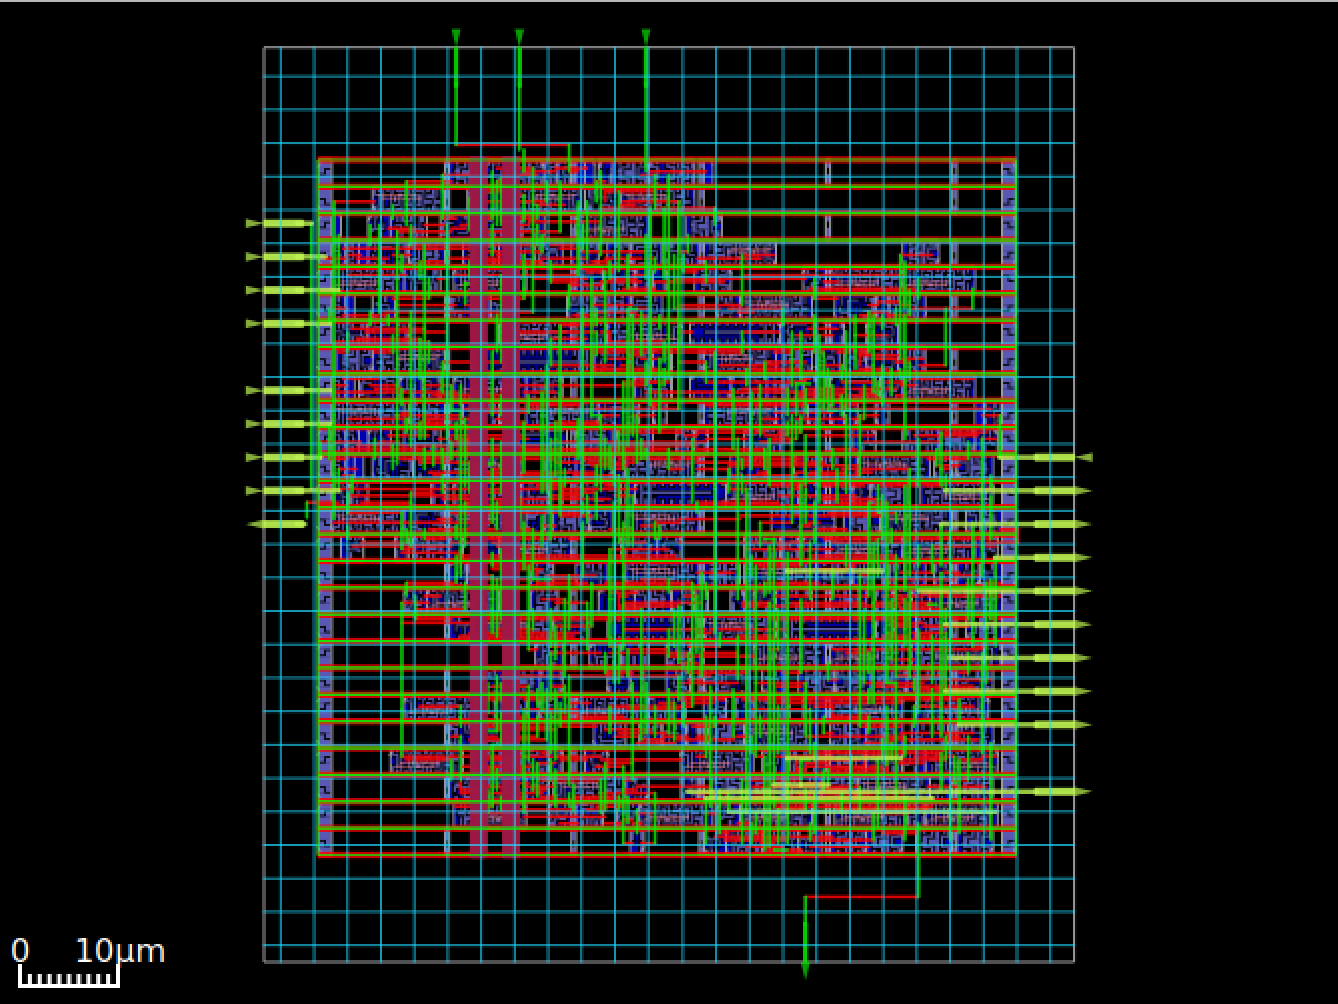
\includegraphics[width=0.93\textwidth]{images/Final_Detailed Routed_Layout_of_the_UART_ASIC.png}
    \caption{Final routed layout generated by OpenROAD.}
    \label{fig:routing}
\end{figure}

The routing stage completed successfully without any congestion or overflow. Table~\ref{tab:routing_metrics} summarizes the routing statistics obtained from the OpenLane2 implementation.

\begin{table}[!htbp]
\centering
\caption{Global and detailed routing statistics}
\label{tab:routing_metrics}
\begin{tabular}{lc}
\toprule
Parameter & Value\\
\midrule
Routed Nets & 314\\
Total Wirelength & 8404 $\mu$m\\
Total Vias & 1804\\
Routing Resource Usage & 14.71\%\\
Routing Overflow & 0\\
Antenna Violating Nets & 0\\
Antenna Violating Pins & 0\\
\bottomrule
\end{tabular}
\end{table}

The routing resource utilization for each metal layer is summarized in Table~\ref{tab:layer_usage}.

\begin{table}[!htbp]
\centering
\caption{Routing resource utilization by metal layer}
\label{tab:layer_usage}
\begin{tabular}{lccc}
\toprule
Layer & Resources & Demand & Usage\\
\midrule
Metal1 & 1406 & 330 & 23.47\%\\
Metal2 & 1428 & 311 & 21.78\%\\
Metal3 & 940 & 17 & 1.81\%\\
Metal4 & 558 & 0 & 0.00\%\\
Metal5 & 140 & 0 & 0.00\%\\
\bottomrule
\end{tabular}
\end{table}

The routing results demonstrate efficient utilization of the available routing resources. The absence of routing overflow confirms that all signal nets were successfully connected without congestion. Furthermore, no antenna violations were reported, indicating that the routing satisfies the manufacturing requirements of the SKY130 process.

%%%%%%%%%%%%%%%%%%%%%%%%%%%%%%%%%%%%%%%%%%%%%%%%%%%%%%%%%%%%%%%

\section{Physical Design Summary}

Table~\ref{tab:physical_summary} summarizes the key results obtained throughout the physical design implementation.

\begin{table}[!htbp]
\centering
\caption{Summary of physical design implementation}
\label{tab:physical_summary}
\begin{tabular}{lc}
\toprule
Metric & Value\\
\midrule
Design Instances & 375\\
Core Area & 5009.80 $\mu m^2$\\
Die Area & 7658.18 $\mu m^2$\\
Core Utilization & 64.09\%\\
Clock Nets & 6\\
Clock Buffers & 5\\
Clock Inverters & 3\\
Timing Repair Buffers & 78\\
Routed Nets & 314\\
Wirelength & 8404 $\mu$m\\
Total Vias & 1804\\
Routing Overflow & 0\\
Antenna Violations & 0\\
\bottomrule
\end{tabular}
\end{table}

The physical implementation of the UART IP core was successfully completed using the OpenLane2 flow. All implementation stages, including floorplanning, placement, clock tree synthesis, and routing, were completed without critical issues. The generated routed layout serves as the input for the physical verification and signoff process presented in the next chapter.